\section{Introduction}\label{section:intro}
The practice of experimental design entails specifying every detail of
running an experiment \cite{chaloner}: at its simplest form,
experimental design involves choosing a set of measurements to be
taken. In a medical experiment, experimental design may involve
choosing participants to whom some drug will be administered, and
measuring their blood pressure. Experimental design also arises 
process of searching for oil. Since measuremnts are expensive and
require digging holes in the ground, only a limited number of
measuremnts can be taken, hence carefully choosing measuremt locations
is crucial.

Specifiyng the right set of measurements holds particular significance
when solving an \emph{inverse problem} --- i.e. making inference of
the physical world utilizing a physical model of some phenomenon of
interest. In an inverse problem, we seek to infer physical quantities,
based on observations and a model of the physical world, typically
phrased in the language of ordinary or partial differential equations.


Inverse problems are ubiquitous in science and engineering, and we
will now give several illustrative examples. In electric impedance
tomography (EIT) we seek to infer the impedance of the inside of a
human body from observations of electrical current impedence measured
at specific electrode locations on the skin, leveraging known
equations of electric current flow
\cite{horesh2010impedance}. Magnetic Resonance Imaging (MRI) also
entails solving an inverse problem, where radio-frequency pulses are
sent through the human body in the presence of a strong magnetic field
and the response of our bodies' contents to such perutrbations is
measured, allowing a radiologist to view the internals of a body in a
noninvasive manner \cite{horesh2008mri}. Yet another example of an
inverse problem arises in oil and gas exploration, where acoustic
waves are sent through "boreholes" --- deep cylindrical wells drilled
into the ground --- and data of travel and return times of said waves
are recorded. Since travel and return time is influenced by the
properties of the subsurface materials, such as density, elasticity,
and the presence of fluids or voids, we can combine travel data with a
geophisical models of contents of the earth's crust to facilitate
reconstructing and inferring the structure of the subsurface in a
process called \emph{borehole tomography}
\cite{horesh2008borehole}. Inverse problems also arise in many other
areas of seismology and geology \cite{rabinowitz1990, steinberg1995}
and medical imaging \cite{tarantola}. Importantly, note that in the
above examples our goal is to infer some function $f \in C(\Omega)$,
where \(\Omega \subseteq \mathbb{R}^d, d=1,2,3\) is a spatial domain
of interest.

%% In EIT, electrode locations determine the quality of the
%% reconstructed impedance field, while in MRI utilizng certain
%% radio-frequency pulses may give more accurate information than
%% others. In borehole tomogrpahy, only several boreholes could be dug
%% and the choice of their locations is also crucial for oil and gas
%% discovery. Thus, the selection of optimal measurements, referred to as
%% the problem of \emph{optimal design}, becomes crucial.
%% in a specific location (in a typical
%% medical application to measure inverventions on, . These experimental
%% units may be individual patients, but also Although common sense is
%% useful in this process, it is often the case that naive intuition
%% results in experiments that do not generate the maximal amount of
%% information possible. To this end

We will now introduce a toy model which we will use to define a toy
inverse problem: the heat equation in one dimension with a homogeneous
Dirichlet boundary condition. The equations are presented below for
completeness, but readers less familiar with partial differential
equations should think of the heat equation as follows: before us
there is a perfectly insulated metal rod. At each point on the rod the
temperature is different, and we call this temperature distribution
the \emph{initial condition}. We wait for a short time and let the
heat dissipate a bit inside the rod. The final heat distribution in
the rod is dictated by the \emph{1D heat equation}:
\begin{subequations}\label{eq:heat equation}
  \begin{alignat}{2}
    u_t &= \Delta u &&\qquad \text{in } [0,1] \times [0,\infty),\\ u
      &= 0 &&\qquad \text{on } \{0, 1\} \times [0,\infty),\\ u &= u_0
        &&\qquad \text{on }[0,1] \times \{0\}.
  \end{alignat}
\end{subequations}

In the inverse problem, our goal is to infer the initial condition
(i.e.~initial temperature distribution inside the rod). We are allowed
to take some number of temperature readings on the rod once our
waiting time has passed. The inverse problem of the 1D heat equation
is difficult ("ill-posed") since heat spreads in a diffusive manner
and any roughness in the initial condition is quickly smoothed, see
Supplementary movies S1 and S2. We will give a fully Bayesian
formulation of this inverse problem in Section \ref{section:prelims}.


In all of the examples of inverse problems we have seen, as well as in
many other applications, measurements should be chosen to most benefit
the user. Hence, the user may consider some utility, called a
\emph{design criterion} and take measurements that maximize this
utility. Two of the most widely recognized and extensively studied
design criteria are A- and D-optimality. We focus on the Bayesian
D-optimality criterion, which carries a simple and intuitive meaning:
measurements chosen according to the D-optimality criterion maximize
the expected Kullback-Liebler divergence from posterior to prior
\cite{Chaloner1995, AlexanderianGloorGhattas14}, see also precise
definition in Section \ref{subsec:D optimal design}. We refer to a set
of measuremnts that maximizes the Bayesian D-optimality criterion a
\emph{D-optimal design}.


Surprisingly, A- and D-optimal designs for inverse problems have been
observed to yield remarkably similar measurements in certain cases
\cite{fedorov1996, nyberg2012, fedorov1997, Ucinski05,
  neitzel2019sparse}. This phenomenon is illustrated for our toy
inverse problem in Fig.~\ref{fig:clusterization illustration}, where
D-optimal measurement locations are shown for different numbers of
measurements. Notably, for six measurements, a D-optimal design yields
two sets of measurements that are almost indistinguishable from one
another. We refer to this intriguing phenomenon as \emph{measurement
clusterization} \cite{Ucinski05}. For our purposes, it suffices for
measurements to be visibly close for clusterization to hold. We refer
to a design that exhibits measurement clusterization as a
\emph{clustered design},


%% first: blue, second: red, third: green, fourth: black,
%% fifth:magenta
\begin{figure}
    \centering
    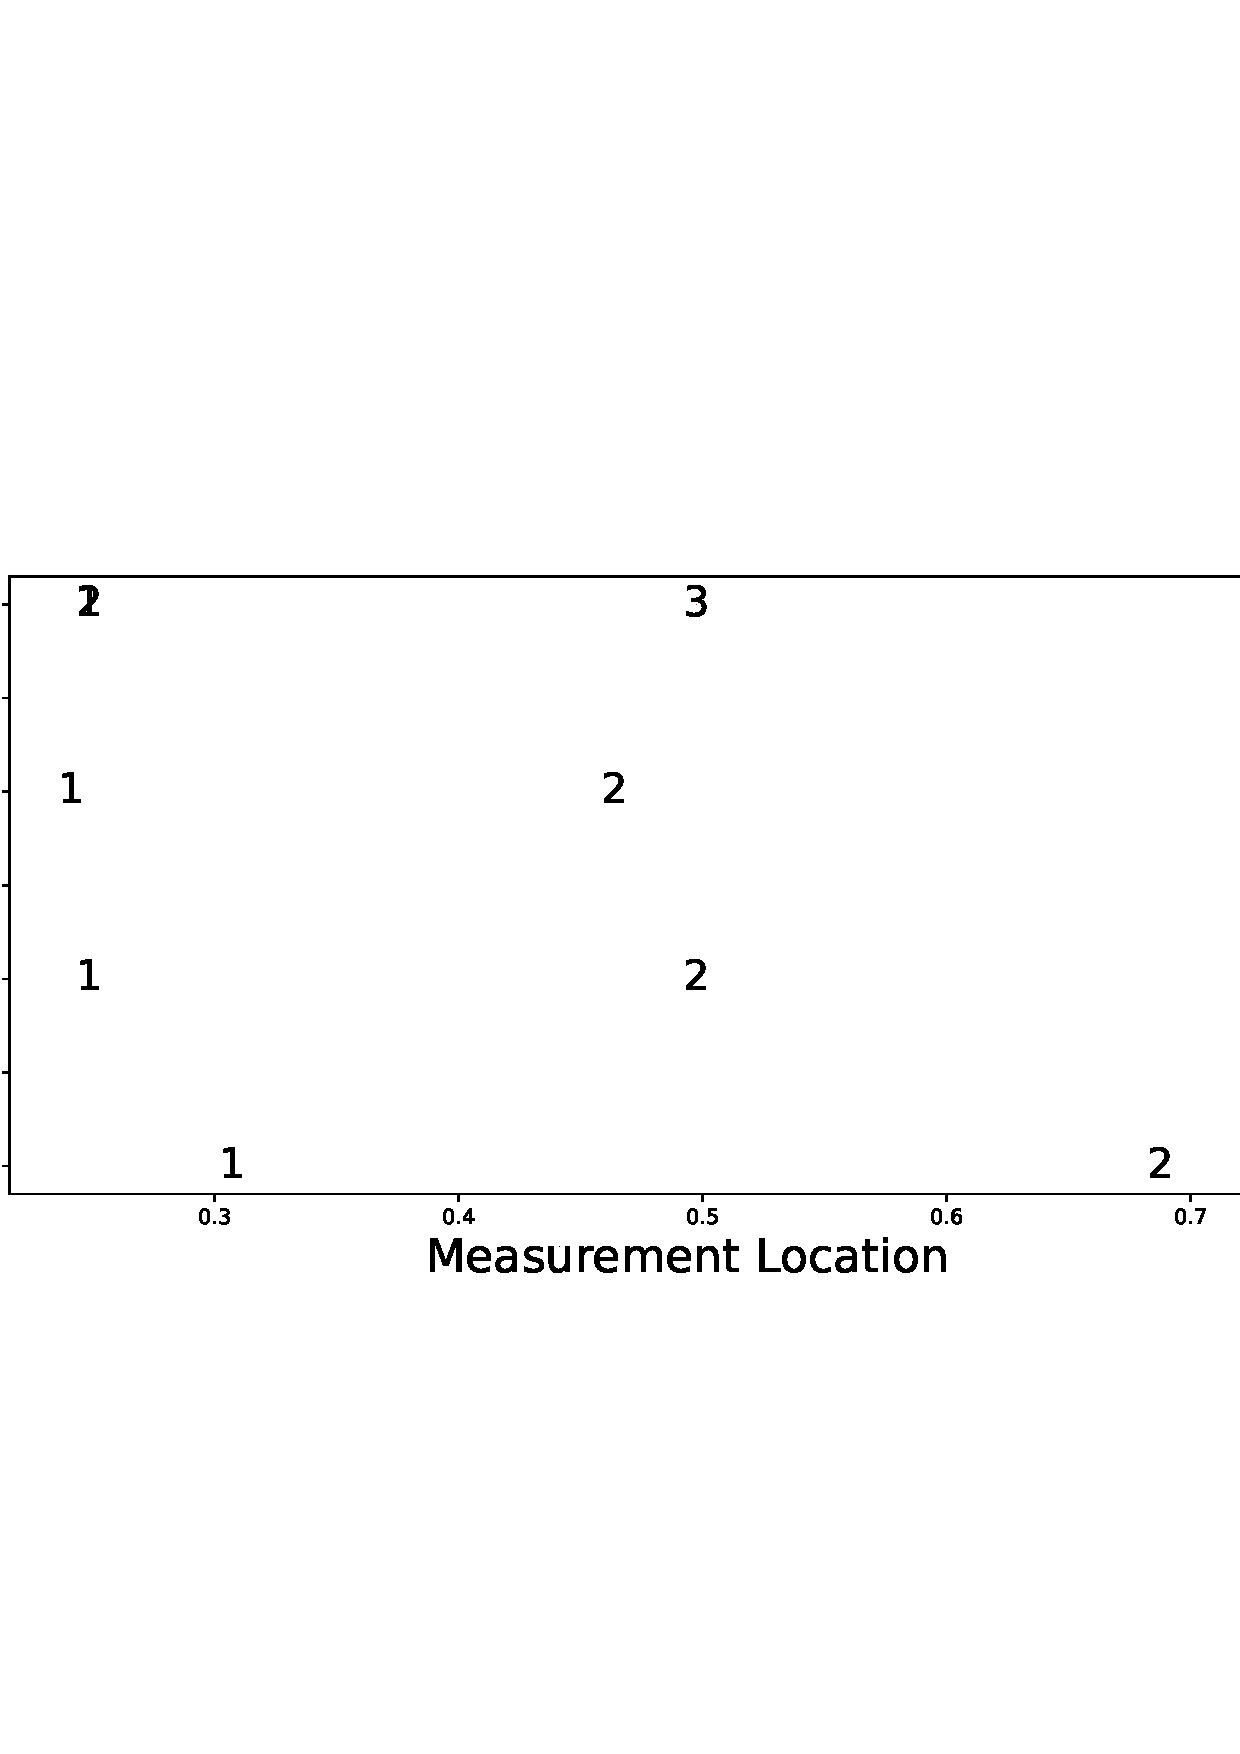
\includegraphics[height=0.5\textwidth]{example.pdf}
    \caption{Measurement clusterization for D-optimal designs for the
      inverse problem of the heat equation. Measurement locations were
      chosen according to the Bayesian D-optimality criterion of
      Theorem \ref{thm:d optimality}. Measurement locations are
      plotted over the computational domain \(\Omega = [0, 1]\)
      (x-axis), for varying numbers of measurements (y-axis). The
      colored numbers are measurement indices, plotted for visual
      clarity. Measurement clusterization already occurs for three
      measurements: the second measurement (red) is overlaid on the
      third (green). For five measurements, first (blue) and second
      (red) measurements are clustered, as well as the fourth (black)
      and the fifth (magenta).}
  \label{fig:clusterization illustration}
\end{figure}

Clusterization should not be confused with either repetition nor with
replication, which are commonly viewed as beneficial and even
necessary aspects of an optimal design \cite{morris, fisher
  schafer2001replication}. For example, in his famous milk and tea
experiment, \cite[Section 11]{fisher} suggested that repetition is a
"way of enlarging the experiment and, thereby, increasing its
sensitiveness". In another example, \cite{fay2000rainfall} measured
the effect of rainfall on grass growth in plots of land. The
experiment involved fifteen "rainfall manipulation shelters", where
"Four rainfall manipulation treatments (three replicates) then were
assigned to 12 of the plots". It seems reasonable the researchers
replicate the phenomenon they are trying to study. Clusterization
seems like a whole different beast: a clustered design in the rainfall
experiment would imply the researchers should take a repeated
measurement \emph{on the same plot}, at the expense of measuring grass
growth in other plots. In sharp contrast to repetition and
replication, clusterization is highly nonintuitive and, as we will
see, its origins run considerably deeper.


Researchers of inverse problems widely agree that measurement
clusterization is undesirable \cite{fedorov1996, nyberg2012,
  fedorov1997, Ucinski05, neitzel2019sparse}, prompting the
exploration of various remedies to address this issue. One approach
involves merging close measurements \cite{fedorov1997}; however, this
strategy merely overlooks the phenomenon of measurement
clusterization. An alternative solution lies in
\emph{clusterization-free design}s, where measurement locations are
deliberately chosen to be distant from one another. This can be
achieved by imposing distance constraints between measurements or by
introducing correlated errors that account for both observation error
and model misspecification \cite{Ucinski05}. For instance, in the
context of time-series analysis for pharmacokinetic experiments,
measurement clusterization can be mitigated by incorporating the
modeling of auto-correlation time within the noise terms
\cite{nyberg2012}.


In spatial problems involving choice of measurements within a domain
\(\Omega \subseteq \mathbb{R}^d, d=1,2,3\), many researchers
circumvent the problem of measurement clusterization by choosing
measurements from a coarse grid in \(\Omega\) \cite{koval2020,
  alexanderian2021, attia2022, alexanderian2014, alexanderian2016,
  alexanderian2018efficient, brunton2016}. This approach incurs a
significant computational cost as it requires solving a difficult
combinatorial optimization problem for measurement locations over a
finite set. The combinatorial optimization problem is usually relaxed
by first assigning optimal measurement weights in \(\mathbb{R}_+\) to
the potential measurement locations. Some researchers incorporate a
sparsifying \(\ell_1\) penalty term into the design criterion, which
is subsequently thresholded to achieve the desired binary design over
the coarse grid \cite{horesh2008borehole}. Others progressively relax
the \(\ell_1\) penalty to an \(\ell_0\) penalty via a continuation
method \cite{alexanderian2016, alexanderian2014}. Others cast the
problem of finding optimal measurement weights as a stochastic
optimization problem \cite{attia2022stochastic}. All of the
aforementioned methods may indeed find a binary optimal design
restricted to a given coarse grid. However, none addresses one
fundamental issue: the restriction of measurement locations to a
coarse grid in \(\Omega\) fundamentally changes the optimal design
problem and thus results in a sub-optimal design.

Avoiding measurement clusterization is a pragmatic approach:
intuitively, researchers recognize that measurement clusterization is
undesirable, even though the underlying reasons may not be fully
clear. Consequently, they strive to prevent it and devise various
methodologies to avoid measurement clusterization. Yet each and every
one of these methodologies achieves its objective by imposing
restrictions on measurement locations, thereby fundamentally altering
the optimal design problem. To the best of my knowledge, no previous
study has tried to address some seemingly simple yet fundamental
questions:
%
Why does imposing correlations between observations alleviate
measurement clusterization?
%
Is measurement clusterization a generic phenomenon? 
%
And, most importantly: Why does measurement clusterization occur?
%
%Should we aim to avoid measurement clusterization?
%
%Is it possible to substitute an optimal clustered design with an
%equally optimal non-clustered design?
%Can an optimal clustered design be relpaced with an equally optimal
%non-clustered design?



\subsection{Contribution}
The primary objective of this study is to provide a comprehensive
understanding of measurement clusterization by addressing the
aforementioned questions. Our focus centers around investigating the
Bayesian D-optimality criterion, which involves maximizing the
expected Kullback-Leibler divergence between the posterior and prior
measures \cite{CoverThomas91, Chaloner1995}. We conduct an analysis of
Bayesian D-optimal designs within the context of linear inverse
problems over Hilbert spaces. We propose a novel relaxed model for
D-optimality that maintains analytical tractability and enables the
identification of D-optimal designs using Lagrange multipliers. This
analytical framework facilitates the exploration of the questions
posed at the end of the previous paragraph:

\begin{figure}
    \centering
    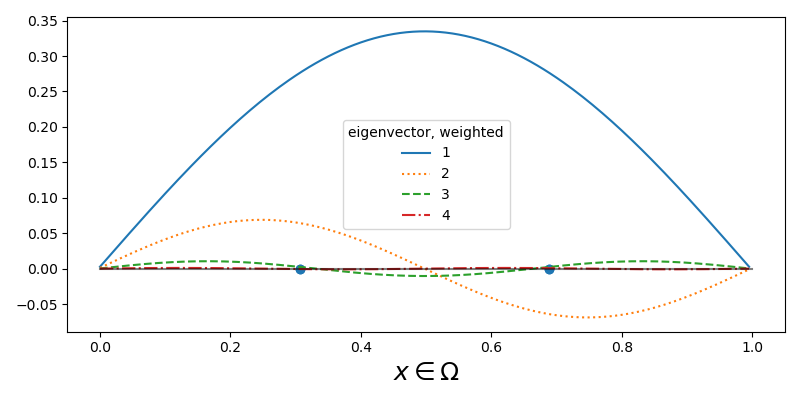
\includegraphics[width=\textwidth]{eigenvectors.pdf}
    \caption{D-optimal measurement locations ($m=4$ measurements) and
      weighted eigenvectors for finding the initial condition of
      the 1D heat equation. Measurement locations and weighted
      eigenvectors are plotted over the computational domain $\Omega =
      [0, 1]$ (x-axis). Measurement clusterization occurs
      approximately at $0.31$ and $0.69$. These two locations are a
      compromise between zeros of eigenvectors a D-optimal design aims
      to ignore (third and up) and staying far from zeros of the
      eigenvectors a D-optimal design aims to measure (first and
      second). Allocating $m=4$ measurements into two locations
      results in clusterization, according to the pigeonhole
      principle.}
  \label{fig:why}
\end{figure}

\begin{enumerate}

\item \label{q:generic} \textbf{Is measurement clusterization a
  generic phenomenon?}
  %\subsection{An answer for Question \ref{q:generic}: Genericity of measurement clusterization}
  %% Computer implementation of Lemma \ref{thm:char} for the inverse
  %% problem outlined in Section \ref{section:how} also generates \(\obs\)
  %% as a solution to the D-optimal design problem.  Furthermore,
  Randomized numerical simulations of our model give rise to D-optimal
  designs that exhibit clusterization more than 95\% of the time (see
  code in supplementary material). Given our model's genericity, we
  expect measurement clusterization to be a generic phenomenon.

\item \label{q:mitigate} \textbf{Why does imposing correlations
  between observations alleviate measurement clusterization?} In
  Section \ref{section:non vanishing}, we rigorously demonstrate the
  role of model error in mitigating clusterization, thereby
  corroborating earlier observations made by various researchers.

\item \label{q:why} \textbf{Why does measurement clusterization
  occur?} In Section \ref{section:why}, we present a compelling
  explanation for the optimality of clustered designs in the absence
  of model error. Our analysis reveals that, in our model, a D-optimal
  design focuses on a select set of prior eigenvectors, specifically
  those with the largest eigenvalues in the prior covariance
  spectrum. In practical scenarios, the number of locations where (a)
  the relevant prior eigenvectors are significantly large, and (b)
  other eigenvectors are close to zero, is limited. Consequently, the
  clusterization of measurements arises as a natural consequence of
  the pigeonhole principle, as there are more measurements available
  than there are locations satisfying conditions (a) and (b). See
  Fig~\ref{fig:why}.


  %% In Section \ref{section:vanishing}, we provide an insightful
  %% explanation for the optimality of clustered designs when no model
  %% error is present. We demonstrate that for our model, a D-optimal
  %% design measures only a small subset of prior eigenvectors, which are
  %% the prior eigenvectors with largest power spectrum. In real-life
  %% problems there are limited number of locations where: (a) the
  %% relevant prior eigenvectors are large, and other prior eigenvectors
  %% with large power in the prior spectrum are zero. Then measurement
  %% clusterization is a result of the pigeonhole principle, where there
  %% are more measurements than measurement locations satisfying (a) and
  %% (b).

  %% We conjecture that the prevalence of measurement clusterization
  %% arises due to the ease of discovering clustered designs.


%% \item \label{q:avoid} \textbf{Should we aim to avoid measurement
%%   clusterization?} Based on the analysis conducted in this study, we
%%   did not find any compelling reason to explicitly avoid optimal
%%   clustered designs.

%% \item \label{q:replace} \textbf{Is it possible to substitute an
%%   optimal clustered design with an equally optimal non-clustered
%%   design?} In Section \ref{section:vanishing}, we answer this question
%%   in the affirmative, although we show that numerical experiments
%%   conducted using our model indicate a strong preference for clustered
%%   designs.

\end{enumerate}

The first insight our study gives is that a D-optimal design aims to
uniformly reduce uncertainties not over space (i.e.~$\Omega$), but
rather over \emph{eigenvectors}. This insight is a part of Theorem
\ref{thm:char}, see Section \ref{section:vanishing} for precise
statement and proof, and see Fig.~\ref{cluste} for an illustration.

In Theorem \ref{thm:char}, we also show that D-optimal designs are
best understood in the sapce of \emph{observations}. Again, a precise
statement could be found in Section \ref{section:vanishing}.  This
result is in accordance with previous work by \cite{koval2020}, who
showed that A-optimal designs are best constructed in the space of
observations.

In the process of proving Theorem \ref{thm:char} we prove and
generalize several lemmas. Among those, is Lemma \ref{lemma:free},
which is a lemma in linear algebra that (to the the best of my
knowledge) is novel: We decompose a symmetric positive definite matrix
\(M \in \mathbb{R}^{k \times k}\) with \(\ttr M = m \in \mathbb{N}\)
as \(M = AA^t\), where \(A\in \mathbb{R}^{k \times m}\) has unit norm
columns.

%% Finally, in Lemma \ref{lemma:lax} we generalize a lemma for
%% calculating \(\frac{\der}{\der t} \log \det (I + X(t))\), where
%% \(X(t)\)is an operator valued function \cite{Lax07}.

Finally, we must stress that we do not suggest that clustered designs
should be abandoned, nor do we support the use of clustered designs in
any circumstances. We merely investigate an intriguing phenomenon of
clusterization and seek a deeper understanding for it. Researchers in
other disciplinesis not viewed as a problem. For example, \cite{lozan}
suggest in the introduction section that repeated measurements are
necessary. Our results align with that common wisdom and settle the
seemed contradiction.


\subsection{Limitations}\label{subsec:limitations}
The main limitation of this study is that our generic model does not
correspond to any specific real-life problem. It is generic enough to
be analytically tractable, but one may argue our model is too far
removed from any real application. To these claims I would answer that
scientists have a long history of studying models that are bare-bones
simplifications of real systems, e.g. the Ising model
\cite{cipra1987}, the Lorenz system \cite{brin}, the Lotka-Volterra
equations \cite{logan2006}, the Carnot engine \cite{kardar2007}, and
many others.
